\documentclass[11pt,a4paper]{article}
\usepackage[a4paper,hmargin=1in,vmargin=1in]{geometry}
\usepackage{pgfplots}
\pgfplotsset{compat=1.17}

\usepackage[czech]{babel}
\usepackage[utf8]{inputenc}
\usepackage[T1]{fontenc}

\usepackage{stddoc}




\begin{document}
\pagenumbering{arabic}


% Needlessly fancy header
    \begin{center}
        \section*{Osnova k výuce přípravných kurzů matematiky}
        \vspace*{-4mm}
        \begin{minipage}{0.4\textwidth}
            \begin{flushleft}
                \textsc{\today}
            \end{flushleft}
        \end{minipage}
        ~
        \begin{minipage}{0.4\textwidth}
            \begin{flushright}
                \textsc{Martin Šimák}
            \end{flushright}
        \end{minipage}
        \noindent\rule{14.5cm}{0.6pt}
    \end{center}


% First lecture
    \section*{Přednáška první}

        \subsection*{Symbolika matematiky}

            V matematice využíváme formální jazyk, který nám umožňuje naše myšlenky a vnitřní logiku našeho uvažování vyjádřit s absolutní precizností. Mluvíme potom o takzvané exaktnosti matematiky, tj. že vyjádření má nulovou míru vágnosti či víceznačnosti. Jedná se proto o prostředek nám práci v akademickém světě ulehčující a nikoliv (jak si mnozí myslí) o prostředek jakési neprostupnosti a šifrování.
            
            Mezi tyto prostředky patří zejména výroky a výrokové formule. O co se jedná? Výroky jsou libovolná tvrzení u nichž má smysl se ptát na jejich pravdivost. Výrokové formule jsou výroky a výroky z nich vzniklé výrokovými spojkami jako např. $\neg, \, \implies$ atd.
            \paragraph{Příklady.}
            \begin{itemize}
                \item Číslo 3 je prvočíslo.
                \item Včera pršelo.
                \item Číšlo 3 je prvočíslo a včera pršelo.
            \end{itemize}

            Výrok může též nabývat pravdivosti v závislosti na nějakém parametru. Například výrok \uv{číslo $x$ je sudé} můžeme označit jako $V(x)$, tedy výrok závislý na parametru $x$. Takové výroky mohou být například rovnice.
            \paragraph{Příklad (BREATHER).}
            Rovnice $x^2 + 1 = 5$ je vlastně výrok v jazyce matematiky, jehož pravdivost závisí na hodnotě parametru $x$.

            Tato souvislost vede přímo na zavedení pojmu množina. Množina je soubor prvků. Takový soubor můžeme definovat buď výčtem jejích prvků nebo charakterizací všech prvků jejich distinktní vlastností. Tato vlastnost je typicky právě výrok nabývající pravdivostní hodnoty 1 právě pro prvky množiny.
            \paragraph{Příklad.}
            \begin{itemize}
                \item $M = \{1,2,3,4,5\}$ je množina,
                \item $N = \{x \in \R \mid x^2 + 1 = 5\}$ je také množina.
            \end{itemize}

            Z toho, jak je zavedena druhá množina (pomocí vlastnosti) můžeme vidět, že je součástí něčeho obecnějšího. V takovém případě mluvíme o podmnožinách. Množina $A$ je podmnožinou množiny $B$ právě tehdy, když pro všechny prvky z A platí, že jsou zároveň i prvky B. Zapisujeme jako $A \subseteq B$. Pokud chceme zdůraznit, že množina $B$ obsahuje i prvky, které v množině $A$ neleží, můžeme vyslovit, že $A$ je vlastní podmnožinou množiny $B$, značíme $A \subset B$. Posledním záklandím pojmem množin je rozdíl množin $B \setminus A$, který obsahuje všechny prvky z $B$ neobsažené v množině $A$.
            \paragraph*{Příklady (POSLEDNÍ JAKO BREATHER OVĚŘIT).}
            \begin{itemize}
                \item Množina $N$ z předchozího příkladu je podmnožinou množiny $\R$, píšeme $N \subseteq \R$, dokonce i $N \subset \R$.
                \item Mějme $A = \{65,12\}$, $B = \{12,47,65\}$, tudíž $A \subset B$ a $B \setminus A = \{47\}$.
                \item Pravdivý výrok $X \subset Y \iff ((X \subseteq Y) \wedge (Y \setminus X \neq \emptyset))$.
            \end{itemize}

            Pomocí vlastnosti být podmnožinou můžeme dále definovat pojem rovnosti množin. Přirozeně tim myslíme indentický obsah obou množin a v matematickém jazyce to zapíšeme jako výrok $A = B \iff (A \subseteq B \wedge B \subseteq A)$.

            Jako poslední ukázku symboliky ještě často používané kvantifikátory $\forall$ a $\exists$ znamenající \uv{pro všechna} a \uv{existuje}
            \paragraph*{Příklady.}
            \begin{itemize}
                \item Výrok \uv{Pro všechna reálná čísla $x$ platí, že druhá odmocnina z $x^2$ je rovna absolutní hodnotě z $x$.} je ekvivalentní s výrokem \uv{$\forall x \in \R : \sqrt{x^2} = |x|$.}
                \item Výše uvedená definice podmnožiny může nabýt formy \uv{$A \subseteq B \iff (\forall y \in A : y \in B)$.}
                \item Definice limity reálné funkce $f$ definované na $D \subseteq \R$ v bodě $x_0$:
                \begin{align*}
                    \lim_{x \to x_0} f(x) = L \iff \forall \epsilon > 0, \, \exists \delta > 0, \, x \in D, \, 0 < |x-x_0| < \delta \Rightarrow 0 < |f(x) - L| < \epsilon.
                \end{align*}
            \end{itemize}

            Nejsofistikovanější a matematiku tvořící výroky jsou axiomy, definice, matematické věty, jejich důkazy a hypotéza.
            \begin{enumerate}[label=(\alph*)]
                \item Axiom je tvrzení, jehož platnost nezpochybňujeme - nedokazují se. Matematika bez nich postrádá smysl, neb nemá na čem stát, z čeho vycházet.
                \item Definice je vymezení matematického pojmu pomocí pojmů základních či dříve definovaných.
                \item Matematická věta je tvrzení, jehož platnost je třeba dokázat.
                \item Důkaz je sled nezpochybnitelných logických postupů zdůvodňujících platnost matematické věty.
                \item Hypotéza je tvrzení s předpokládanou platností, avšak kompletní důkaz není poskytnut. Je možno ji tedy potvrdit či vyvrátit.
            \end{enumerate}

            Ačkoli techniku důkazu nelze generalizovat na všechny věty, existuje pro spcifické případy pár postupů, jejichž procedura (je-li aplikovatelná) je korektní, viz důkaz sporem či matematická indukce.

        \subsection*{Taky něco spočtěme}
            
            \begin{enumerate}

                \item Rozehřívačka:
                \begin{enumerate}[label=(\alph*)]

                    \item převod kvadratické funkce $f(x) = 4x^2 - 5x + 1$ na čtverec (5 min):
                    \begin{align*}
                        f(x) &= 4x^2 - 5x + 1 = 4 \( x^2 - \frac 54 x + \frac 14 \) = 4 \( x^2 - \frac 54 x + \frac{25}{64} - \frac{25}{64} + \frac 14 \) =
                    \\
                        &= 4 \( x^2 - \frac 54 x + \frac{25}{64} \) - \frac{25}{16} + 1 = 4 \( x - \frac 58 \)^2 - \frac{9}{16}.
                    \end{align*}

                    \item řešení rovnice $f(x) = 0$, kde $f$ je kvadratická funkce z předchozího příkladu (5 min):
                    \begin{enumerate}[label=(\roman*)]

                        \item mechanické řešení:
                        \begin{align*}
                            4x^2 - 5x + 1 &= 0,
                        \\
                            x_{1,2} &= \frac{5 \pm \sqrt{25 - 4 \cdot 4}}{8},
                        \\
                            x_{1,2} &= \frac{5 \pm 3}{8},
                        \\
                            x &\in \left\{-\frac 14; 1 \right\}.
                        \end{align*}

                        \item řešení za použití předchozího výsledku:
                        \begin{align*}
                            4 \( x - \frac 58 \)^2 - \frac{9}{16} &= 0,
                        \\
                            \( x - \frac 58 \)^2 &= \frac{9}{64},
                        \\
                            x - \frac 58 &= \pm \frac{3}{8},
                        \\
                            x_{1,2} &= \frac{5 \pm 3}{8},
                        \\
                            x &\in \left\{-\frac 14; 1 \right\}.
                        \end{align*}

                    \end{enumerate}
                \end{enumerate}

                \item Obecná kvadratická rovnice $ax^2+bx+c=0$ a jak ji vyřešit. Mechanické řešení umí, vyřešit bez apriorní znalosti řešení (10-15 min):
                \begin{align*}
                    ax^2 + bx + c &= 0, \quad a \neq 0,
                \\
                    a\( x^2 + \frac ba x + \frac ca \) &= 0,
                \\
                    x^2 + \frac ba x + \frac{b^2}{4a^2} - \frac{b^2}{4a^2} + \frac ca &= 0,
                \\
                    x^2 + \frac ba x + \frac{b^2}{4a^2} &= \frac{b^2}{4a^2} - \frac ca,
                \\
                    \( x + \frac{b}{2a} \)^2 &= \frac{b^2 - 4ac}{4a^2},
                \\
                    x + \frac{b}{2a} &= \pm \frac{\sqrt{b^2 - 4ac}}{2a}, \quad \Big/ \text{ správně abs}
                \\
                    \Aboxed{x_{1,2} &= \frac{-b \pm \sqrt{b^2 - 4ac}}{2a}.}
                \end{align*}

            \end{enumerate}
    
    \section*{Přednáška druhá}
        
        \subsection*{Funkce}

            Zobrazení $f$ z množiny $A$ do množiny $B$: taková binární relace, která každému prvku z množiny $A$ přiřadí nejvýše jeden prvek z $B$.\\
            * Binární relace je pojem popisující vztah prvků z jedné množiny k prvkům z množiny druhé (například $\leq$, $>$, $=$, "být sourozenec" atd.).\\
            Pro nás důležité hlavně reálné funkce: Reálná funkce je zobrazení $f: M \to \R$, kde $M$ je libovolná neprázdná podmnožina reálných čísel. Dále definujeme pojmy:
            \begin{itemize}
                \item definiční obor funkce $D(f)$ jako množinu $M$,
                \item obor hodnot $H(f)$ je podmnožina $\R$ obsahující všechna reálná čísla, které mohou vzniknout jako obraz funkce $f$.
            \end{itemize}

            \noindent
            Dále u funkcí určujeme základní vlastnosti:
            \begin{itemize}
                \item omezenost zdola: funkce $f$ je omezená zdola právě tehdy, když existuje $K$ tak, že pro všechna $x \in D(f)$ platí $f(x) \geq K$,
                \item omezenost shora: funkce $f$ je omezená shora právě tehdy, když existuje $L$ tak, že pro všechna $x \in D(f)$ platí $f(x) \leq L$,
                \item absolutní omezenost: řekneme, že funkce $f$ je omezená, pokud existuje $M$ tak, že pro všechna $x \in D(f)$ platí $|f(x)| \leq M$,
                \item sudost: $\forall x \in D(f) : f(-x) = f(x)$,
                \item lichost: $\forall x \in D(f) : f(-x) = -f(x)$,
                \item růst na $G \in D(f)$: $\forall x,y \in G : (x < y \implies f(x) < f(y))$,
                \item klesání na $G \in D(f)$: analogicky.
            \end{itemize}

            \subsubsection*{Lineární a afinní funkce}
                Linearita: $\forall x,y \in D(f), \, \alpha,\beta \in \R : f(\alpha x + \beta y) = \alpha f(x) + \beta f(y)$.
                Lineární funkce jsou tedy funkce $f(x) = ax$, funkce $f(x) = ax + b$ je afinní. Nakreslit grafy. Funkce jsou neomezené, monotónní, lineární jsou liché.
                \paragraph*{Příklady.}

                \paragraph*{Intermezzo: Absolutní hodnota.} Význam a graf absolutní hodnoty. Jak nám absolutní hodnota změní charakter lineárních rovnic a nerovnic (příklady).

            \subsubsection*{Mocninné funkce}
                $f(x) = a x^n$, kde $a \in \R$ a $n \in \N \setminus \{1\}$. Nakreslit grafy. Liché mocniny jsou liché funkce, sudé jsou sudé. Odtud název parity.

            \subsubsection*{Kvadratické funkce}
                \begin{itemize}
                    \item Obecný předpis $f(x) = a x^2 + bx + c = a(x-x_V) + y_V$, kde $[x_V,y_V] = V$ a $a \neq 0$, graf.
                    \item Vlastnosti: $D(f) = \R$, $(-\infty, y_V]$ nebo $[y_V, \infty]$ v závislosti na vedoucím parametru $a$. Pokud vrchol leží na ose y ($x=0$), pak je to sudá funkce. Je vždy bď zdola nebo shora omezená.
                \end{itemize}
                \paragraph*{Příklady.} Nakreslit graf, určit průsečíky s osama, převést na čtverec, odvození kvadratické formule, kvadratické rovnice, nerovnice.
                
    \section*{3/9/2021}
        \begin{itemize}
            \item Opakování sami a pak na tabuli: neúplné kvadratické rovnice, vzorec, vztahy mezi kořeny (Viet, rozklad).
        \end{itemize}

    \section*{3/11/2021}
        \begin{itemize}
            \item Opakování víceméně samostatně: kvadratická funkce $f(x) = 4x^2 -20x - 24$ -> převést na čtverec -> kořeny $f(x) = 0$ -> součinový tvar -> ověření Vietových vzorců. Na tabuli graf.
            \begin{align*}
                f(x) &= 4 (x - 5/2)^2 - 49,
            &
                K &= \left\{ -1, 6 \right\}.
            \end{align*}

            \item Hlubší opáčko: dvě rovnice s absolutními hodnotami.
            \item Povídání: kvadratický trojčlen (pokecat o rozdílem mezi funkcí a rovnicí, co to vlastně znamená ted předpis, co kterým zkoumat), průbehy funkcí.
            \item Příklady sami rychle: kvadratický trojčlen (příklad na průběh, rozklad na součin).
            \item Kvadratické nerovnice, jejich význam (výrok), příklady.
            \item Další příklady na kvadratické rovnice a nerovnice (rozložený kvartický rovnice, absolutní hodnota).
            \item Pokud zbyde čas: společná úloha o pohybu.
        \end{itemize}

    \section*{4/1/2021}
        \begin{itemize}
            \item Pokec + opakování, co jsme dělali na minulých hodinách.
            \item Hodina fyzikálních aplikací.
            \item Rovnoměrně přímočarý pohyb jako lineární funkce.
            \item Úloha o pohybu vedoucí na kvadratické rovnice.
            \item Přirozený způsob nárůstu a poklesu jako exponenciální funkce, například nervové vnímání a reakce mozku.
            \item Logaritmus aplikovaný na široké škály a na veličiny v exponenciálním tvaru: hladina akustického tlaku, přenosy obvodů (analogové filtry, návrh domácích stereí).
        \end{itemize}

    \section*{4/15/2021}
        
        \subsection*{Trigonometrie, úhly a oblouková míra}
        \begin{itemize}
            \item Scio příklad.
            \item Pokecat o motivaci goniometrických funkcí: pozorování, že všechny pravoúhlé trojúhelníky s jedním úhlem $\alpha$ mají stejné poměry stran.
            \item Zavedení gonio fcí, základní gonio identity.
            \item Argument gonio fcí úhel, pokecat o obloukové míře jako vhodné a přirozené náhradě úhlů z $s = \varphi r$.
            \item Uvést přepočetní vztahy.
        \end{itemize}

    \section*{4/20/2021}

        \subsection*{Goniometrické funkce}
        \begin{itemize}
            \item Jednotková kružnice, pravoúhlé trojúhelníky v ní a goniometrické funkce jako souřadnice. Zatim jenom sinus, kosinus.
            \item Ukázat si určování hodnot na běžných úhlech $0,\pi/6,\pi/4,\pi/3,\pi/2,2\pi/3,3\pi/4,5\pi/6$ z jednotkové kružnice. Důraz na orientovaný úhel.
            \item Popovídat o úhlech $\theta \not\in [0,2\pi]$ $\rightarrow$ rotace do stejných hodnot sinu a kosinu $\rightarrow$ periodičnost g.f. + definice periodické funkce.
            \item Vykreslit význačné hodnoty do grafu a spojit do hladké funkce sinus, kosinus.
            \item Promluvit o vlastnostech funkcí sinus a kosinus. Ukázat, jak jsou vidět už na jednotkové kružnici, e.g. periodičnost, parity.
        \end{itemize}
        \begin{figure}[!htb]
            \centering
            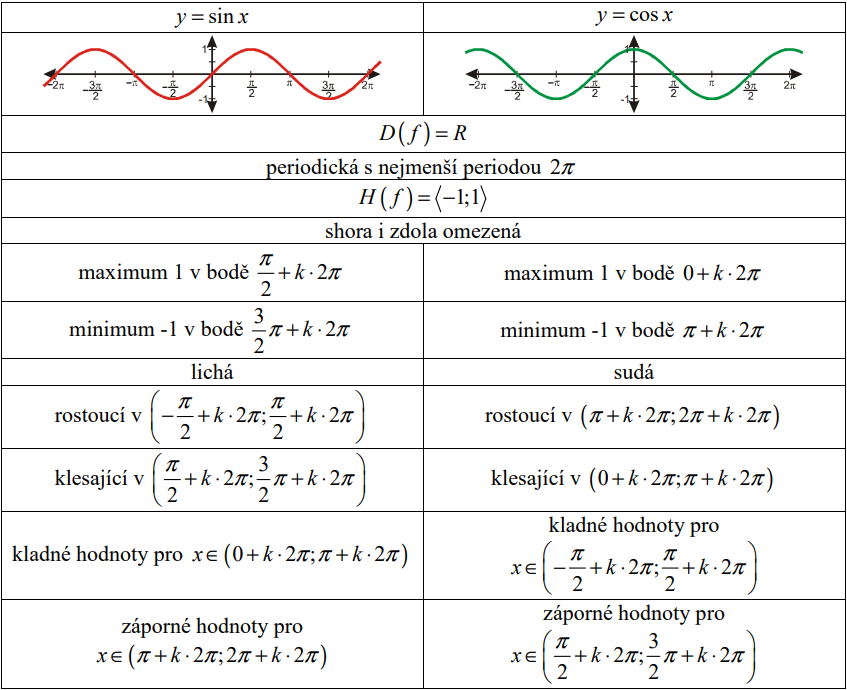
\includegraphics[width=0.75\textwidth]{figs/gf-tab.png}
            \caption{Tabulka sin,cos}
        \end{figure}

    \section*{4/22/2021}
        
        \begin{itemize}
            \item Grafické příklady.
        \end{itemize}

    \section*{4/27/2021}

        \begin{itemize}

            \item Zavedení tangenty a kotangenty podíly sinu a kosinu. Grafy, vlastnosti, jednotková kružnice.
            
            \item Základní vzorce a odkud se vzaly: unitární identita sinu a kosinu z Pythagora v jednotkové kružnici, parity again, periodické posuvy, symetrie sinu a kosinu:
            \begin{align*}
                \sin^2(x) + \cos^2(x) &= 1,
            &
                \tan(x) \cdot \cot(x) &= 1,
            \\
                \sin(x) &= \cos\(x-\frac \pi 2\),
            &
                \cos(x) &= \sin\(x + \frac \pi 2\),
            \\
                \sin\(x+\pi\) &= -\sin(x),
            &
                \cos\(x+\pi\) &= -\cos(x),
            \\
                \cot(x) &= \tan\(-x+\frac \pi 2\).
            \end{align*}

            \item Bez důkazu součtové vzorce a vzorce dvoujnásobného argumentu:
            \begin{align*}
                \sin(x+y) &= \sin(x)\cos(y) + \cos(x)\sin(y),
            &
                \sin(x-y) &= \sin(x)\cos(y) - \cos(x)\sin(y),
            \\
                \cos(x+y) &= \cos(x)\cos(y) - \sin(x)\sin(y),
            &
                \cos(x-y) &= \cos(x)\cos(y) + \sin(x)\sin(y),
            \\
                \sin(2x) &= 2\sin(x)\cos(x),
            &
                \cos(2x) &= \cos^2(x) - \sin^2(x),
            \\
                \sin^2(x) &= \frac{1-\cos(2x)}{2},
            &
                \cos^2(x) &= \frac{1+\cos(2x)}{2},
            \\
                \left| \sin\(\frac x2\) \right| &= \sqrt{\frac{1-\cos(x)}{2}},
            &
                \left| \cos\(\frac x2\) \right| &= \sqrt{\frac{1+\cos(x)}{2}}.
            \end{align*}

            \item Goniometrické rovnice:
            \begin{align*}
                \sin(x) &= 0,
            \\
                \cos(x) &= -\frac12,
            \\
                \sin(x) &= -\frac{\sqrt 3}{2},
            \\
                \sin(x) &= 0,1,
            \\
                1-(\sin(x)-1) &= 2-\sqrt 3\(\sqrt 3 \sin(x) - 1\),
            \\
                \frac{\cos(x) + \cos(\pi)}{\sin\(7\pi/6 \)\cos(x)} &= \sin\(\frac \pi 2\) + 1,
            \\
                2\sin^2(x) + 3\sin(x) - 2 &= 0.
            \end{align*}

        \end{itemize}
        \begin{figure}[!htb]
            \centering
            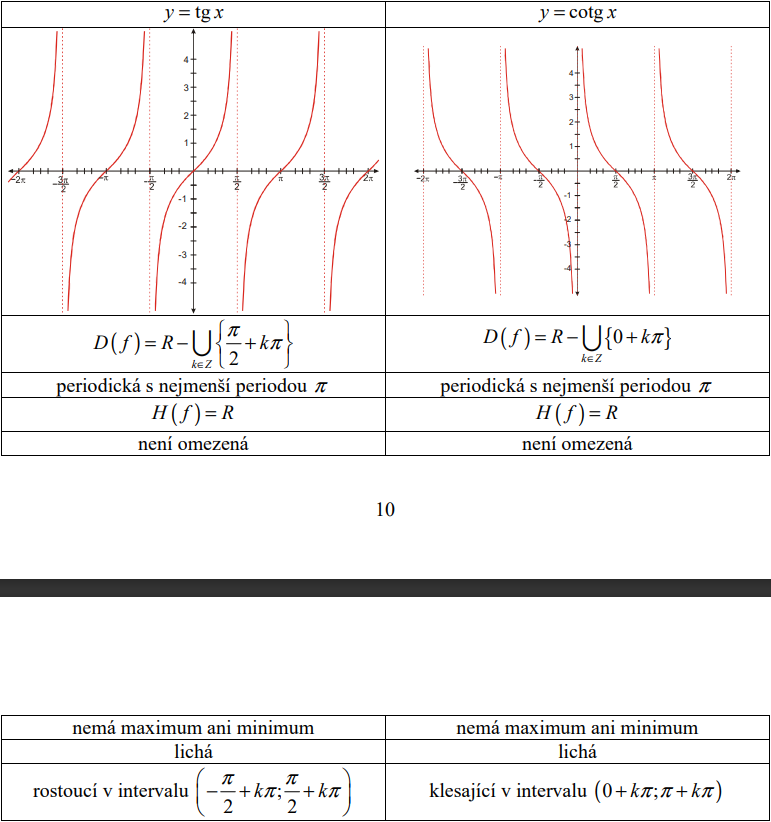
\includegraphics[width=0.75\textwidth]{figs/tan-cot.png}
            \caption{Tabulka tan,cot}
        \end{figure}

    \section*{11/5/2021}
        \begin{itemize}
            \item Posloupnosti na přání
            \item Pořešit bonusovou hodinu na integrály
            \item Poděkovat za elegantní mail Iloně
        \end{itemize}
        \subsection*{Komplexní čísla}
        \begin{itemize}
            \item Zatím neintuitivní zavedení komplexní jednotky $i$. Motivace rozšíření číselného oboru, možnost řešení polynomiálních rovnic. Možná trochu historie.
        \end{itemize}

    \section*{13/5/2021}
        \begin{itemize}
            \item Geometrie přímky pomocí reálných čísel (translace součtem, škálování násobením, zrcadlení/reflexe násobením $(-1)$).
            \item Let's get back to $i \times i = i^2 = -1$. Provedení stejné operace dvakrát činí reflexi. Co to znamená? Základní geometrická transformace: rotace. Reflexe je rotace o $\pi$, tj. násobení $i$ je rotace o $\pi/2$.
            \item Ukázka toho, co je to $i^k$, kde $k \in \{1,2,3,4\}$. Spočítat i ukázat pomocí rotací.
            \item Podotknout, že komplexní rovina je $\R^2$ vybavená specifickým násobením vektorů jako rotace.
            \item Srovnání reálných a komplexních čísel (vyjádření pomocí jednoho desetiného rozvoje vs. páru rozvojů, bod na přímce vs. bod v rovině)
            \item Procvičení aritmetiky (reálná a imaginární část, kvadrát komplexního čísla, komplexní sdružení, definice absolutní hodnoty komplexních čísel)
        \end{itemize}

    \section*{18/5/2021}
        \begin{itemize}
            \item Procvičování: algebraický tvar $(1+i):(2-i)$.
            \item Pozor: Neověřili jsme, že je vůbec možné každému komplexnímu číslu $z$ najít inverzi $1/z$.
            \item Kvadratická rovnice s komplexním kořenem
            \begin{align*}
                x^2-2x+10=0.
            \end{align*}
            \item Hele: řešením je komplexní číslo a jeho komplexní sdružení. Platí, že pokud $z$ je kořen, tak $\bar z$ taky obecně?
            \item Ověřit větu „Je-li součin dvou komplexních čísel roven nule, je rovno nule alespoň jedno z nich.“
            \item Algebraický $\rightarrow$ goniometrický tvar komplexních čísel, komplexní sdružení v goniometrickém tvaru.
            \item Zopakování absolutní hodnoty a ukázat, že komplexně sdružená čísla mají stejnou absolutní hodnotu.
            \item Důkaz pravidel pro výpočet absolutních hodnot $|z_1\cdot z_2|$ a $|z_1/z_2|$.
        \end{itemize}

    \section*{20/5/2021}
        \begin{itemize}
            \item Opakovní z konce minulé hodiny: goniometrický tvar z algebraického (popis jednotkové a nejednotkové kružnice).
            \item Násobení a dělení komplexních čísel v goniometrickém tvaru.
            \item Moiverova věta, možnost jednoduché komputace $z^n$, mocninné a odmocninné funkce.
            \item Ukázka Eulerovy identity, exponenciální tvar komplexních čísel, nejkrásnější rovnice matematiky.
            \item Euler nahradil součtové vzorce. Odvodit tedy součtové goniometrické vzorce z Eulera.
            \item Co obecně geometricky znamená násobit dvě komplexní čísla? Obecná rotace v rovině (goniometrický a exponenciální tvar).
            \item Pomocí rotací můžeme získat smysl dříve známých pravd o komplexních číslech: $z \bar z = |z|^2$, rotace o $\pi/2$ násobením $i$ a $i^2 = -1$.
        \end{itemize}

    \section*{27/5/2021}

\newpage
        \begin{enumerate}
            \item \begin{align*}
                y[n+3] + n^2 y[n] &= \frac{1}{n+1}.
            \end{align*}
            Systém je diskrétní, lineární, časově invariantní a neautonomní.

            \item \begin{align*}
                y''(t) + y(t) &= \sin(t), \quad y(0) = -1, \, y'(0) = 3,
            \\
                p^2Y(p) - py(0) - y'(0) + Y(p) &= \frac{1}{1+p^2},
            \\
                (p^2+1)Y(p) &= -p+3 + \frac{1}{p^2+1},
            \\
                Y(p) &= \frac{-p+3+\frac{1}{p^2+1}}{p^2 + 1},
            \\
                Y(p) &= \frac{(3-p)(p^2+1) + 1}{(p^2+1)^2},
            \\
                H(p) &= \frac{Y(p)}{U(p)} = \frac{\frac{(3-p)(p^2+1) + 1}{(p^2+1)^2}}{\frac{1}{p^2+1}},
            \\
                H(p) &= \frac{(3-p)(p^2+1) + 1}{p^2 + 1} = \frac{(3-p)(p^2+1)+1}{(p+i)(p-i)}.
            \end{align*}
            Jak je vidět, máme kořeny $\pm i$. Oba mají reálnou složku nulovou, a tak je systém na mezi stability.

            \item \begin{align*}
                y[n+2]-y[n] &= n, \quad y[0] = -1, \, y[1] = 1, \, n \in \N_0,
            \\
                z^2\(Y(z) - y[0] - \frac{y[1]}{z}\) - Y(z) &= \frac{z}{(z-1)^2},
            \\
                (z^2-1)Y(z) &= -z^2 + z + \frac{z}{(z-1)^2},
            \\
                Y(z) &= \frac{-z^2+z+\frac{z}{(z-1)^2}}{z^2-1} = \frac{(z-z^2)(z-1)^2+z}{(z^2-1)(z-1)^2},
            \\
                H(z) &= \frac{Y(z)}{U(z)} = \frac{\frac{(z-z^2)(z-1)^2+z}{(z^2-1)(z-1)^2}}{\frac{z}{(z-1)^2}},
            \\
                H(z) &= \frac{(z-z^2)(z-1)^2+z}{z(z^2-1)} = \frac{(z-z^2)(z-1)^2+z}{z(z-1)(z+1)}.
            \end{align*}
            Opět vidíme, že kořeny systémové funkce leží ve dvou případech ($\pm 1$) na jednotkové kružnici a jeden (0) leží uvnitř. Celkově tak máme závěr, že systém je opět na mezi stability.
        \end{enumerate}

        

        




        
\newpage
        \section*{Někdy jindy - polynomy}
            Obecně (polynom $n$-tého řádu) se jedná o funkci
                \begin{align*}
                    P_n(x) = a_n x^n + a_{n-1} x^{n-1} + \cdots + a_1 x + a_0 = \sum_{k=0}^n a_k x^k.
                \end{align*}
            Tyto polynomy jsou velkou součástí úvodního matematického předmětu lineární algebra (strašák prváků). Proto je vhodné si připomenout pár základních vlastností. Násobení polynomů člen po členu (klasické roznásobování závorek), stupeň polynomu jakožto nejvyšší mocnina, dělení polynomů, kořen polynomu a jeho násobnost.

            Dělení polynomu polynomem: Mějme dva nenulové polynomy $a(x)$ a $b(x)$, které chceme navzájem podělit jako $a(x) : b(x)$. Můžeme proto (bez důkazu) napsat, že výsledek bude vypadat jako
            \begin{align*}
                a(x) &= q(x) \cdot b(x) + r(x),
            \end{align*}
            kde $q(x)$ (kvocient) a $r(x)$ (zbytek) jsou polynomy a $r(x)$ má menší stupeň než $b(x)$.

            \noindent \emph{Příklad}, třeba $(x^3 - 2x^2 + 2x - 1):(x-3)$ a $(x^3 - 2x^2 + 2x - 1):(x-1)$. Pozorování: číslo $x_0 = 1$ je kořen děleného polynomu $\to$ dělení vyšlo beze zbytku. Náhoda? Let's see.

            Dále můžeme říci, že máme-li polynom $a(x)$, můžeme jeho hodnotu v bodě $x_0$ spočítat jako zbytek po dělení polynomu $a(x)$ závorkou $(x-x_0)$. Opravdu: pokud vezmeme v potaz výše napsané tvrzení, dostáváme, že hodnota polynomu je
            \begin{align*}
                a(x_0) = (x-x_0) \cdot q(x) + r(x) \Big|_{x=x_0} = r(x_0).
            \end{align*}
            Navíc speciálně, pokud je $x_0$ kořen polynomu (tj. $a(x_0) = 0$), musí platit
            \begin{align*}
                a(x_0) = (x-x_0) \cdot q(x) + r(x) \Big|_{x=x_0} = r(x_0) \overset != 0,
            \end{align*}
            tedy že platí $r(x_0) = 0$. Z věty o dělení polynomu polynomem ale máme, že zbytek musí být polynom menšího řádu než je řád polynomu, kterým dělíme. To je v našem případě $(x-x_0)$, tj. polynom 1. řádu, a tak $r(x)$ musí být konstanta (polynom nultého řádu). Víme tedy, že polynom $r(x)$ je vlastně konstanta a má nulovou hodnotu. Odvodili jsme tak takzvanou \emph{kořenovou faktorizaci}, kdy polynom $n$-tého řádu s $n$ kořeny (včetně násobností) můžeme rozdělit na součin $n$ tzv. kořenových faktorů, tj. dvojčlenů $(x-x_k)$, kde $x_k$ je $k$-tý kořen polynomu. Toto platí pro všechny polynomy $n$-tého řádu. Hlavní věta algebry totiž praví, že polynom $n$-tého řádu má $n$ komplexních kořenů. V reálném oboru to vždycky jít nemusí.

            \noindent\emph{Příklad}, rozložit $p(x) = x^6 - 3x^4 + 2x^3$ na součin kořenových faktorů.

\end{document}